\documentclass[11pt,usenames,dvipsnames,aspectratio=169]{beamer}
%\usetheme{cern}
\usetheme{cernomc}

% Beamer Setup ---
\setbeamercovered{transparent=5} 
\setbeamertemplate{navigation symbols}{} 

\AtBeginSection{%
	\begin{frame}[noframenumbering]{Outline}
	\tableofcontents[currentsection]
	\end{frame}
}

% Imports ---
\usepackage[utf8]{inputenc}
\usepackage{amsmath}
\usepackage{amsfonts}
\usepackage{amssymb}
\usepackage{mathtools}
\usepackage{bm}  % bold math
\usepackage{graphicx}
\usepackage{grffile}  % filenames with dots 
\usepackage{tikz}
\usepackage{hyperref}
\usepackage{siunitx}
\usepackage{booktabs}
\usepackage{multirow}
\usepackage{caption}
\usepackage[absolute,overlay]{textpos}

% some shenanigans -------------------------------------------------------------
\newcommand{\highl}[1]{\textbf{#1}}
\definecolor{RunTwored}{RGB}{200,0,0}
\definecolor{APJgreen}{RGB}{20,150,0}
\definecolor{SbSorange}{RGB}{240,150,0}


% Meta -------------------------------------------------------------------------
\author[OMC]{%
Andreas Wegscheider on behalf of the OMC team\\%
% hacky, I know ...
\centering%
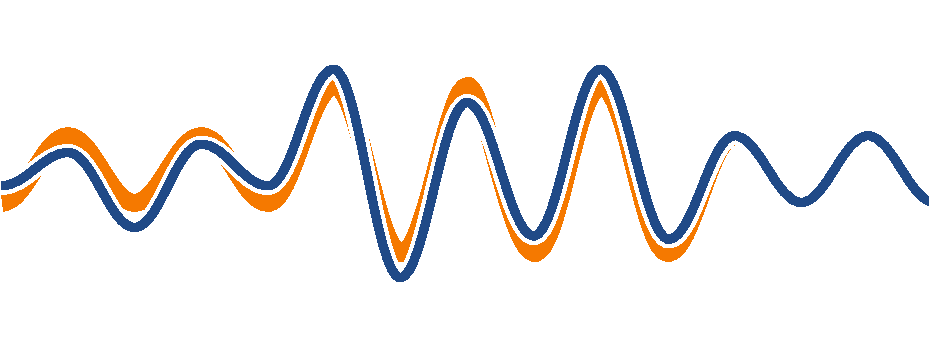
\includegraphics[width=3cm]{omc-logo.pdf}%
}
\title[LHC 2022]{LHC Commissionning 2022}
\logo{} 
\titlegraphic{}
\institute{CERN}
\date[09.06.22]{09.06.2022}
\subject{} 

% Document ---------------------------------------------------------------------
\begin{document}

\begin{frame}
    \titlepage
\end{frame}


\begin{frame}{Full Outline}
\tableofcontents
\end{frame}


\small

\section{The Way to Top Energy}

% Injection --------------------------------------------------------------------


\begin{frame}{Injection optics}
    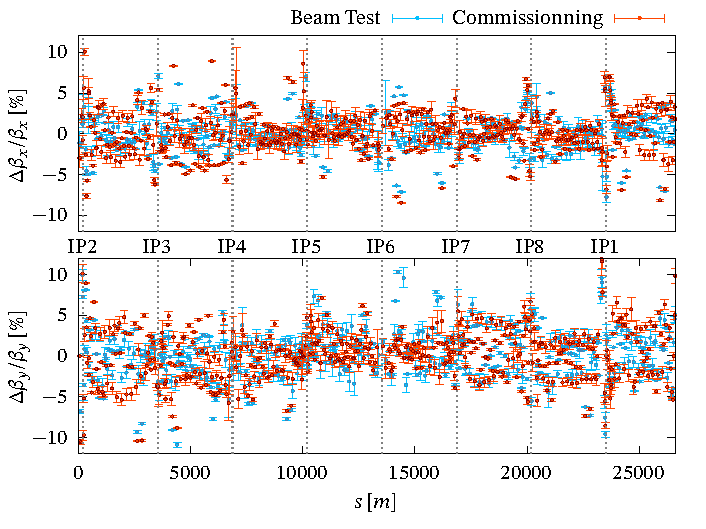
\includegraphics[width=0.49\linewidth]{images/beamtest/b1_bb.pdf}
    \hfill
    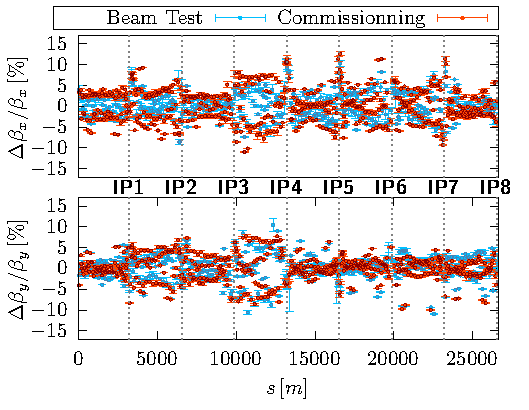
\includegraphics[width=0.49\linewidth]{images/beamtest/b2_bb.pdf}
    
    \begin{itemize}
        \item  Measured the injection optics with the corrections of \highl{2021 beam test}.
        \item Looks similar, \highl{no corrections} were re-calculated.
    \end{itemize}
\end{frame}


% Ramp -------------------------------------------------------------------------


\begin{frame}{Coupling in the Ramp}
    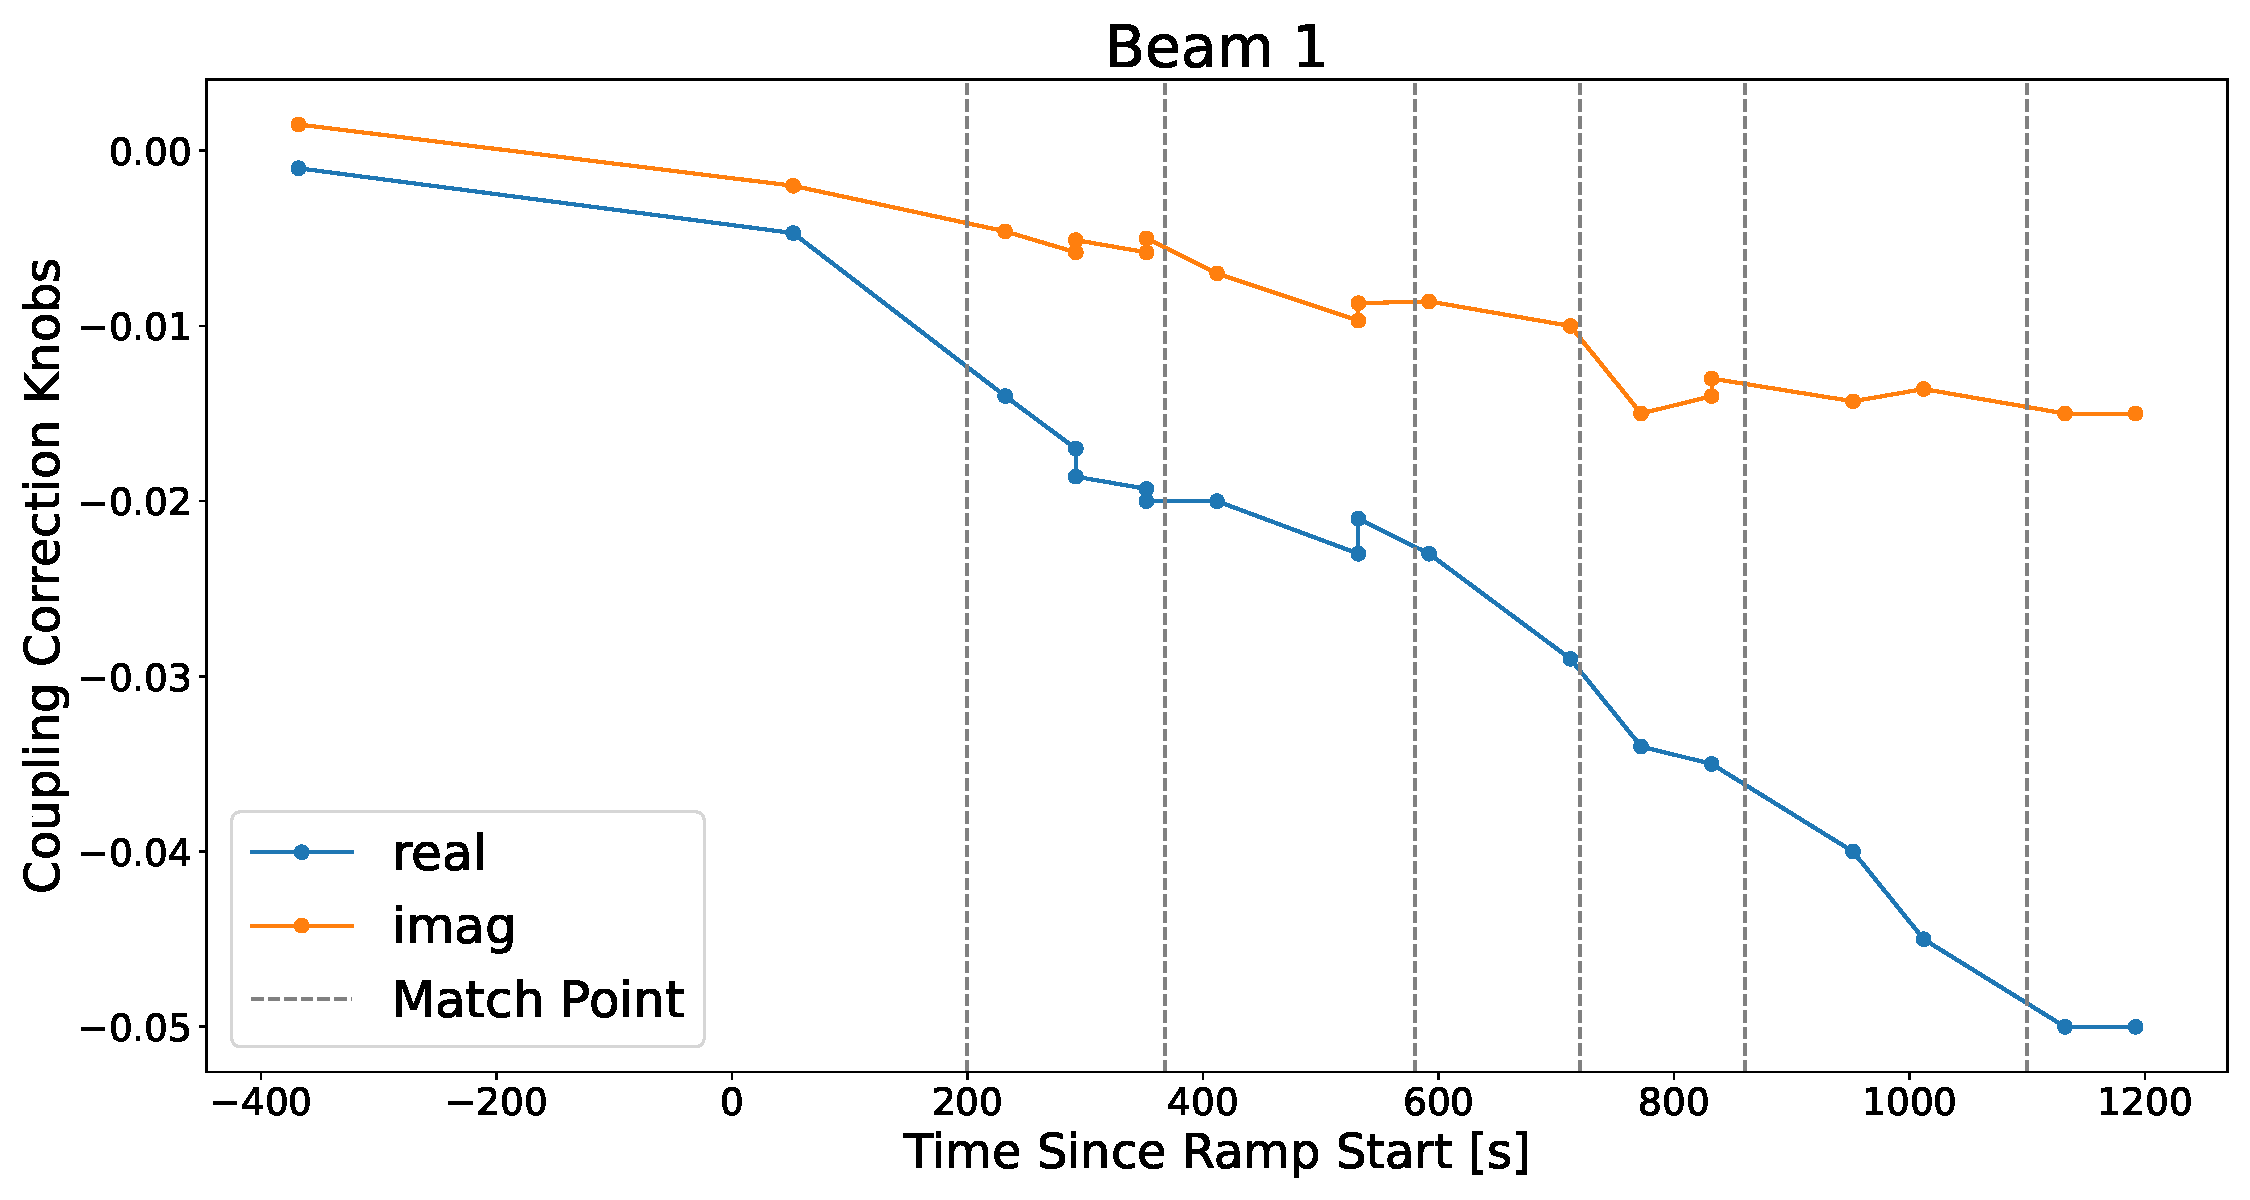
\includegraphics[width=0.49\linewidth]{images/ramp/B1_coupling_correction_knobs_in_ramp.pdf}
    \hfill
    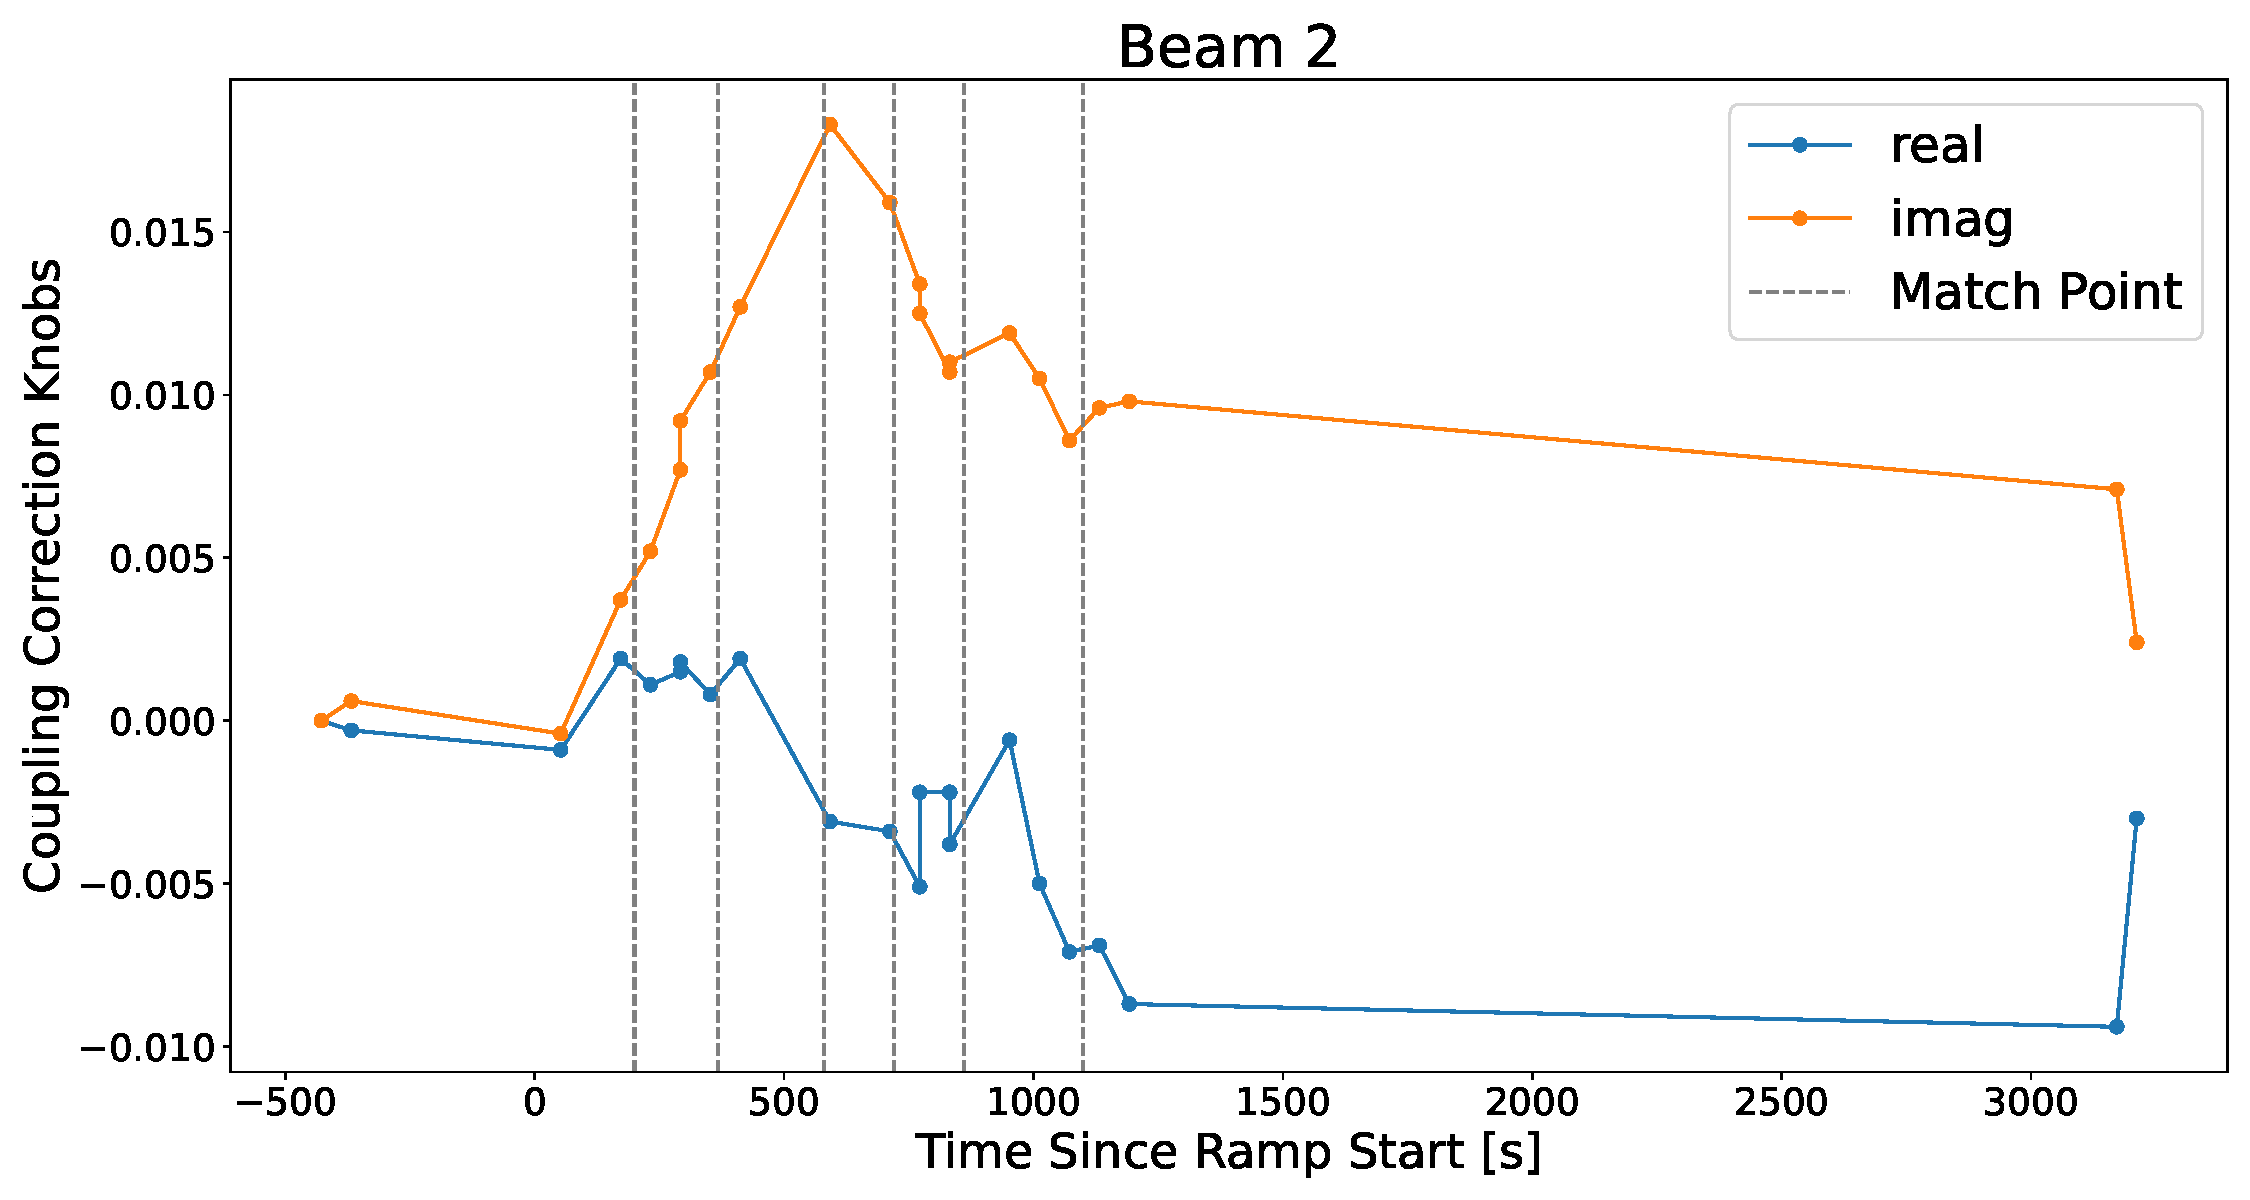
\includegraphics[width=0.49\linewidth]{images/ramp/B2_coupling_correction_knobs_in_ramp.pdf}
    
    \begin{itemize}
        \item %
            did \highl{manual coupling} measurement during the ramp because the coupling server
            \highl{failed to give} good results 
        \item %
            calculated \highl{coupling corrections} (verifying on the way that the selected model didn't deteriorate the calculations)
        \item %
            these were \highl{programmed in} to be applied during the next ramp
        \item %
            re-measure showed that we corrected \highl{$< 0.005$ at every pick-up point}
    \end{itemize}
\end{frame}


% Flattop ---------------------------------------------------------------------


\begin{frame}{Flattop}
    
    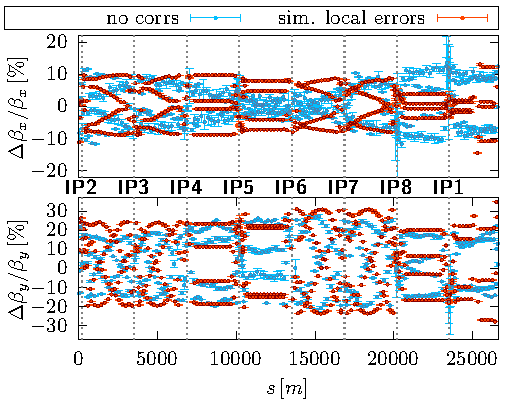
\includegraphics[width=0.49\linewidth]{images/flattop/b1_bb.pdf}
    \hfill
    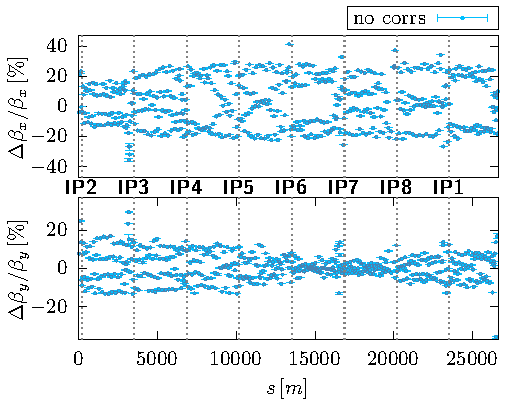
\includegraphics[width=0.49\linewidth]{images/flattop/b2_bb.pdf}
    \begin{itemize}
        \item measurements at \SI{6.8}{TeV} performed
        \item errors within tolerances, no dedicated corrections
    \end{itemize}
    
\end{frame}

\section{Squeeze}


\begin{frame}{\SI{30}{cm} Optics -- record high $\beta$~beating}

    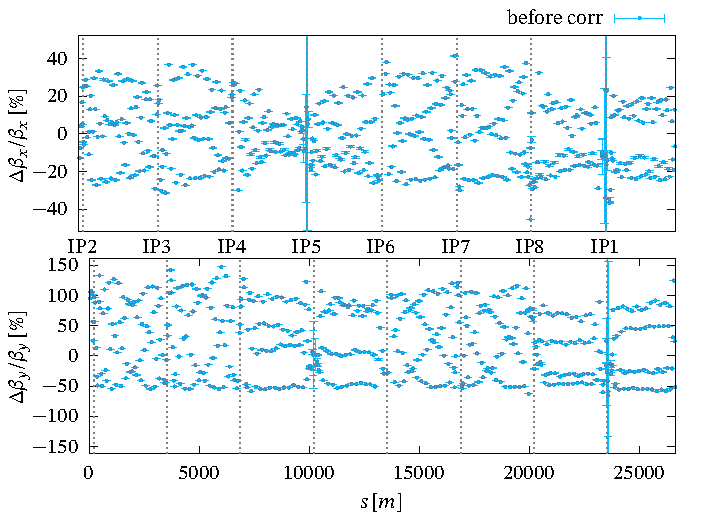
\includegraphics[width=0.49\linewidth]{images/squeeze/b1_recordhigh.pdf}
    \hfill
    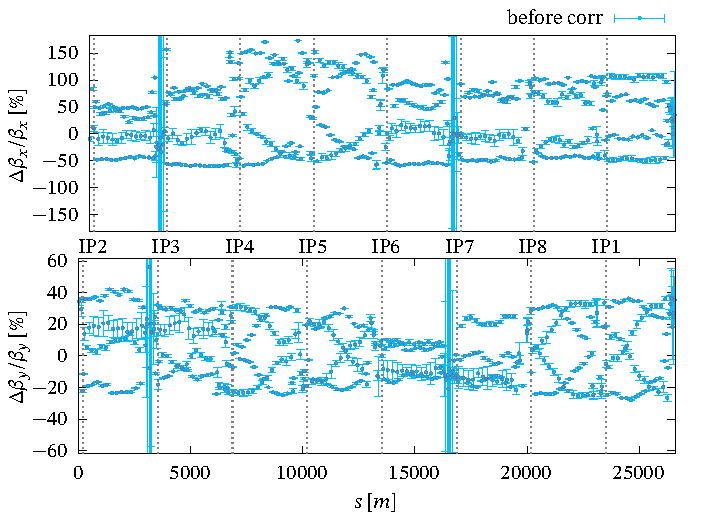
\includegraphics[width=0.49\linewidth]{images/squeeze/b2_recordhigh.pdf}
    
    \begin{itemize}
        \item peak $\beta$~beating of \textbf{150 \%}
        \item highest ever measured in the LHC
    \end{itemize}
    
\end{frame}


\begin{frame}{30cm Optics \only<1>{-- Beam~1}\only<2>{-- Beam~2}}
    \begin{center}
        \only<1>{
            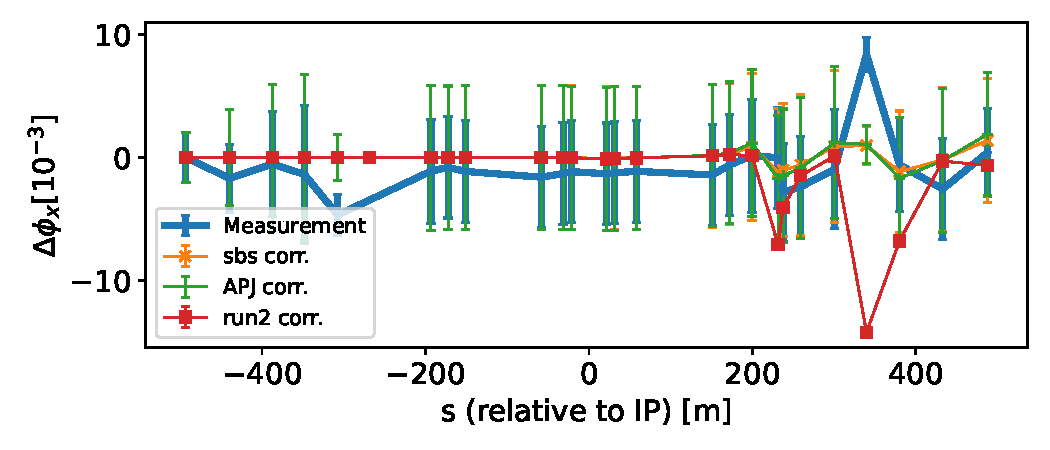
\includegraphics[width=0.4\linewidth]{images/flattop/beam1_x_IP1.pdf}
            \hspace{1cm}
            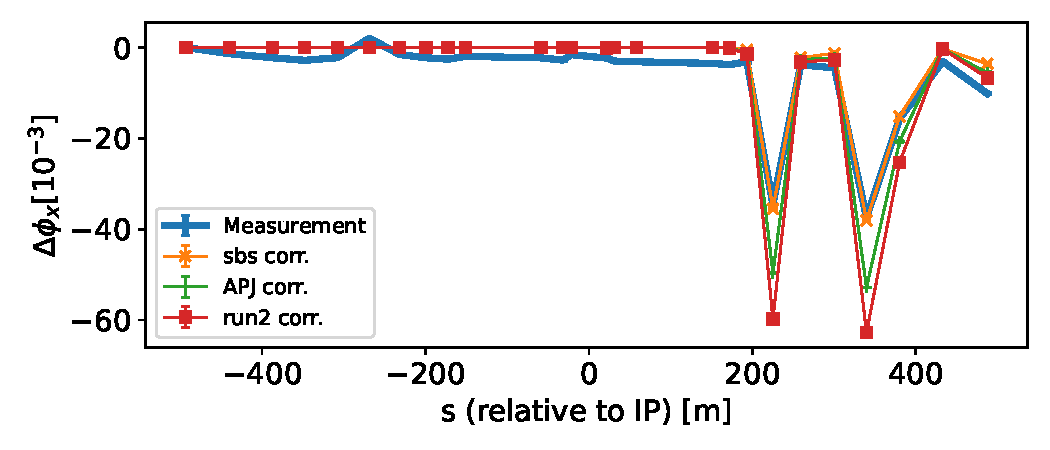
\includegraphics[width=0.4\linewidth]{images/flattop/beam1_x_IP5.pdf}
            \\
            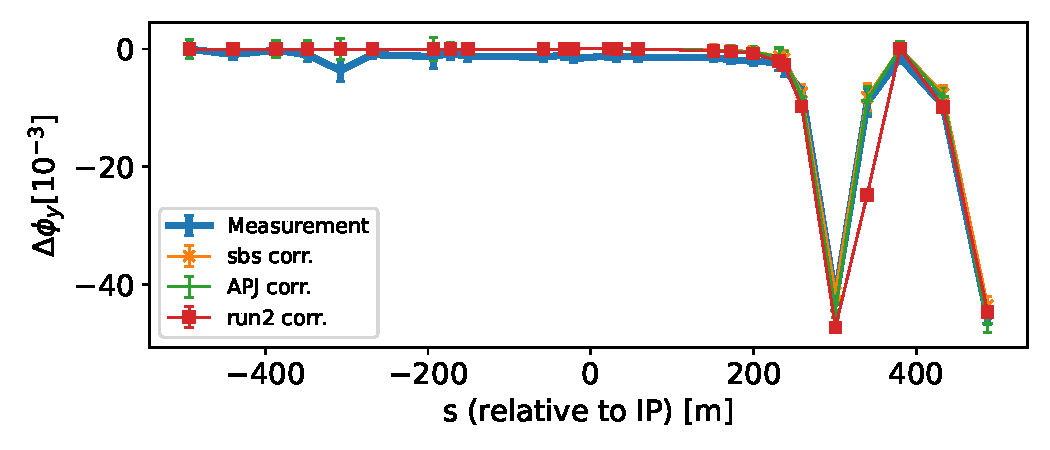
\includegraphics[width=0.4\linewidth]{images/flattop/beam1_y_IP1.pdf}
            \hspace{1cm}
            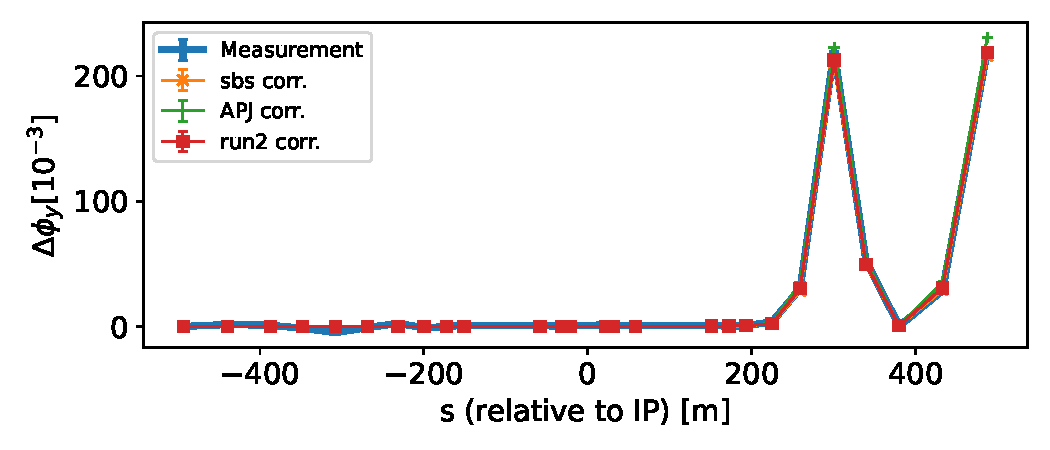
\includegraphics[width=0.4\linewidth]{images/flattop/beam1_y_IP5.pdf}
        }
        \only<2>{
            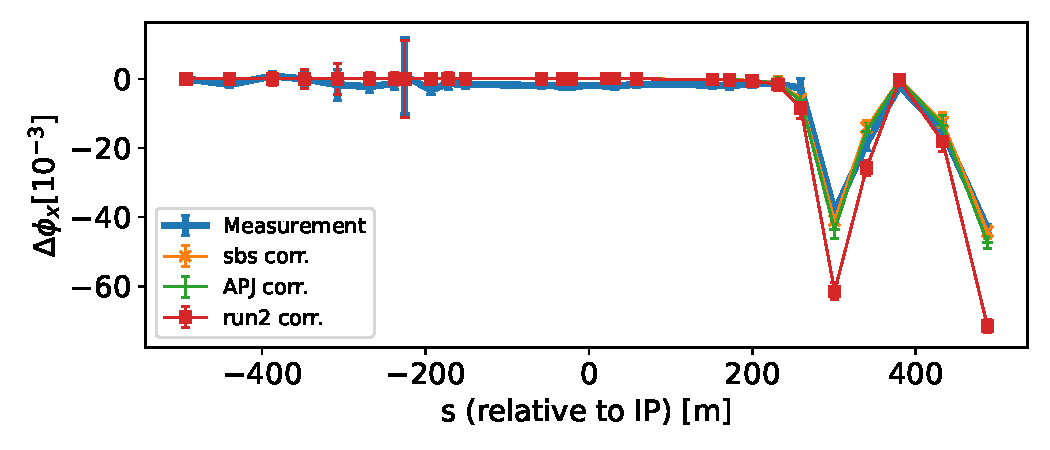
\includegraphics[width=0.4\linewidth]{images/flattop/beam2_x_IP1.pdf}
            \hspace{1cm}
            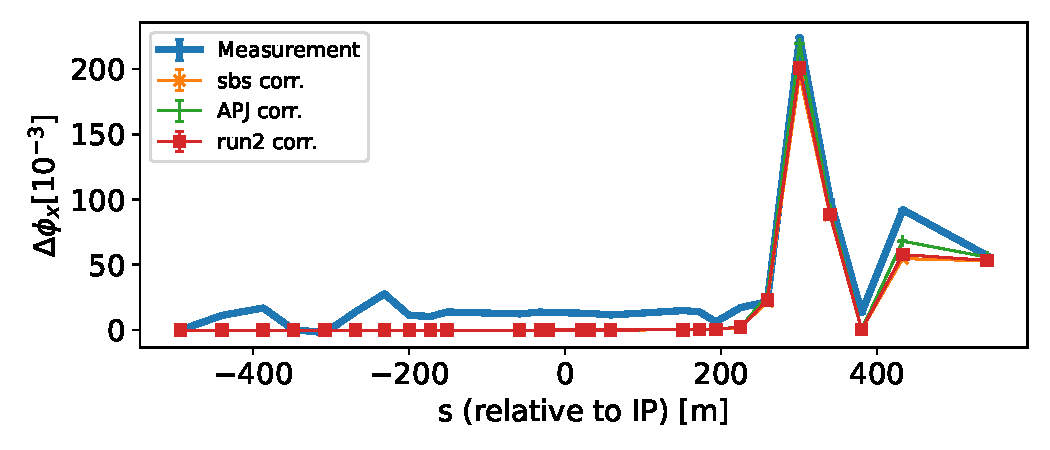
\includegraphics[width=0.4\linewidth]{images/flattop/beam2_x_IP5.pdf}
            \\
            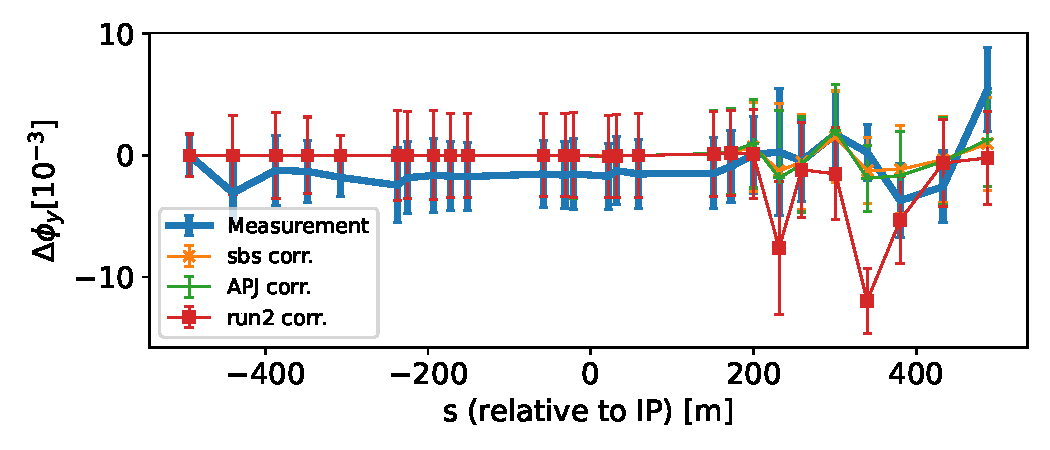
\includegraphics[width=0.4\linewidth]{images/flattop/beam2_y_IP1.pdf}
            \hspace{1cm}
            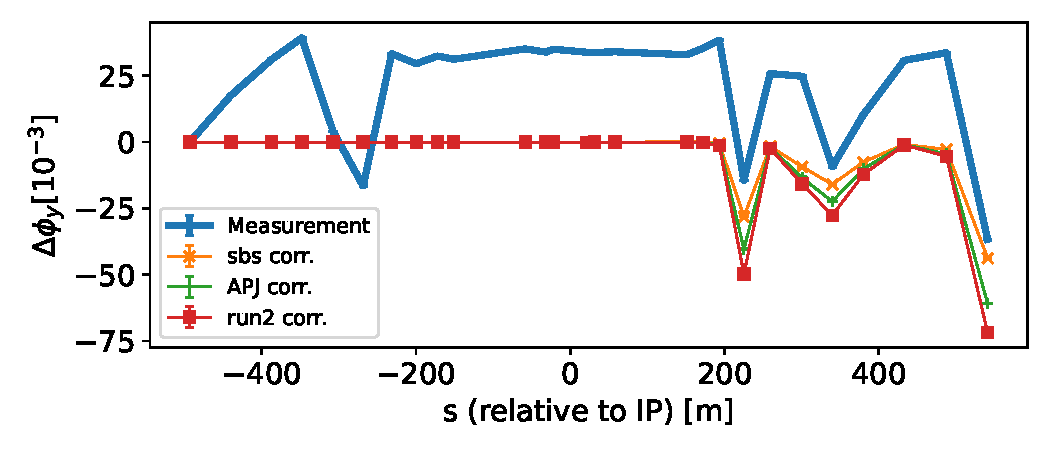
\includegraphics[width=0.4\linewidth]{images/flattop/beam2_y_IP5.pdf}
        }
        \only<3>{
        {\tiny
         \begin{tabular}{l|lSSS|c|} \toprule
              & \textbf{Circuit}%
              & \multicolumn{3}{c|}{$\Delta k (10^{-5}\SI{}{m^{-2}})$}
              & \textbf{Polarity}%
              \\ \cmidrule{2-6}
              &
              & \multicolumn{1}{c}{\color{RunTwored}\textbf{Run 2}} &{\color{APJgreen}\textbf{APJ}} &{\color{SbSorange}\textbf{SbS}}
              & \textbf{LSA} \\\hline \midrule
     IR1 & \texttt{ktqx1.l1} & \color{RunTwored} 1.23 & \color{APJgreen} 0    & \color{SbSorange} 1.23 & - \\
         & \texttt{ktqx1.r1} & \color{RunTwored}-1.23 & \color{APJgreen} 0    & \color{SbSorange}-1.23 & + \\
         & \texttt{ktqx2.l1} & \color{RunTwored} 0.65 & \color{APJgreen} 1.15 & \color{SbSorange} 0.41 & + \\
         & \texttt{ktqx2.r1} & \color{RunTwored}-1.0  & \color{APJgreen}-0.87 & \color{SbSorange}-0.70 & - \\
         & \texttt{ktqx3.l1} & \color{RunTwored} 1.22 & \color{APJgreen} 1.94 & \color{SbSorange} 1.22 & - \\
         & \texttt{ktqx3.r1} & \color{RunTwored}-1.22 & \color{APJgreen}-2.88 & \color{SbSorange}-1.22 & + \\\hline \midrule
     IR5 & \texttt{ktqx1.l5} & \color{RunTwored} 2.0  & \color{APJgreen} 0    & \color{SbSorange} 2.25 & - \\
         & \texttt{ktqx1.r5} & \color{RunTwored}-2.0  & \color{APJgreen} 0    & \color{SbSorange}-2.10 & + \\
         & \texttt{ktqx2.l5} & \color{RunTwored} 0.26 & \color{APJgreen} 0.38 & \color{SbSorange} 0.16 & + \\
         & \texttt{ktqx2.r5} & \color{RunTwored} 1.48 & \color{APJgreen} 0.93 & \color{SbSorange} 1.35 & - \\
         & \texttt{ktqx3.l5} & \color{RunTwored} 1.49 & \color{APJgreen} 3.40 & \color{SbSorange} 2.25 & - \\
         & \texttt{ktqx3.r5} & \color{RunTwored}-1.49 & \color{APJgreen}-2.46 & \color{SbSorange}-2.10 & + \\\hline \midrule
        \end{tabular} 
        }
        }
    \end{center}
    \begin{itemize}
        \item measurements at $\beta^*=\SI{30}{\centi\meter}$ performed
        \item corrections calculated using \highl{APJ}, \highl{SbS} and taken from \highl{run2}
        \item APJ and SbS yield \highl{similar results} when applied,
            run2 corrections are over-correcting
    \end{itemize}
\end{frame}


\begin{frame}{\SI{30}{cm} Optics -- before and after local corrections}

    \begin{center}
    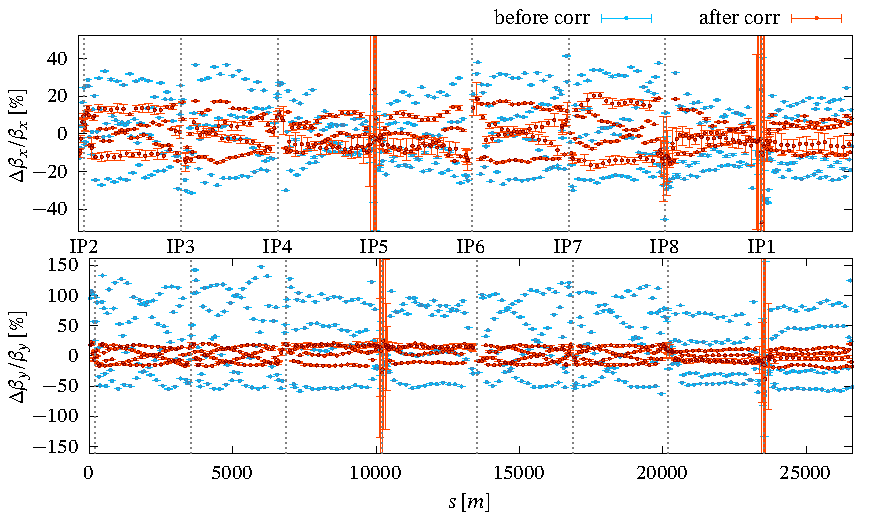
\includegraphics[width=0.49\linewidth]{images/squeeze/b1_bb_comp.pdf}
    \hfill
    
\includegraphics[width=0.49\linewidth]{images/squeeze/b2_bb_comp.pdf}
    \end{center}
    
    \begin{itemize}
        \item $\beta$~beating \highl{after implementation} of local corrections in IPs \textbf{1}, \textbf{2}, \textbf{5} and \textbf{8}
        \item IP1 correction is taken from \highl{APJ}, others from \highl{SbS}
        \item $\beta$~beating stays \highl{under 20\%}
    \end{itemize}
    
\end{frame}


\begin{frame}{\SI{30}{cm} Optics -- before and after global corrections}

    \begin{center}
    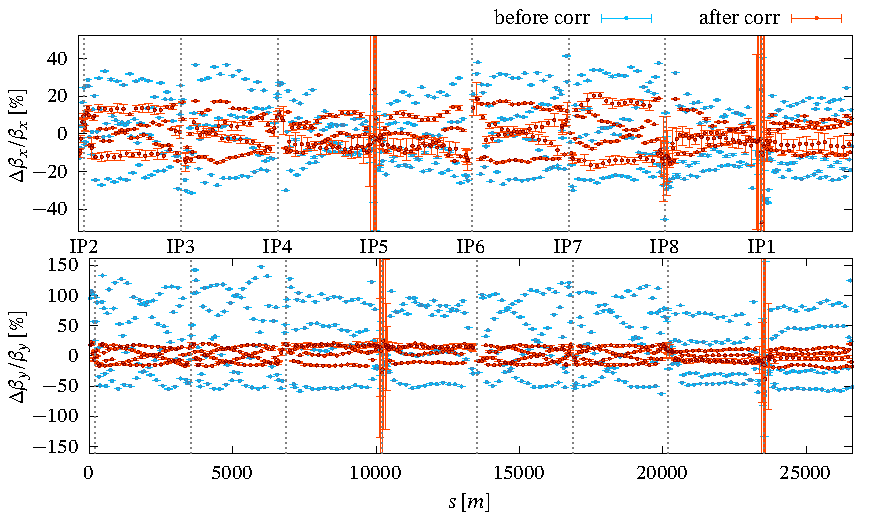
\includegraphics[width=0.49\linewidth]{images/squeeze/b1_bb_comp.pdf}
    \hfill
    
\includegraphics[width=0.49\linewidth]{images/squeeze/b2_bb_comp.pdf}
    \end{center}
    
    \begin{itemize}
        \item $\beta$~beating \highl{after implementation} of local corrections in IPs \textbf{1}, \textbf{2}, \textbf{5} and \textbf{8}
        \item IP1 correction is taken from \highl{APJ}, others from \highl{SbS}
        \item $\beta$~beating stays \highl{under 20\%}
    \end{itemize}
    
\end{frame}


% Ballistic -------------------------------------------------------------------
\section{Ballistic}
\begin{frame}{Ballistic Optics}
    
\end{frame}


% Non-Linear ------------------------------------------------------------------
\section{Non-linear optics}


\begin{frame}{Chromaticity}
    \begin{itemize}
        \item $Q''$ agrees with beam test, $Q'''$ does not
        \item $Q'''$ corrected in a first step
        \item $Q'''$ and $Q''$ corrected in second iteration
    \end{itemize}
\end{frame}


\begin{frame}{Amplitude Detuning}
    \begin{center}
        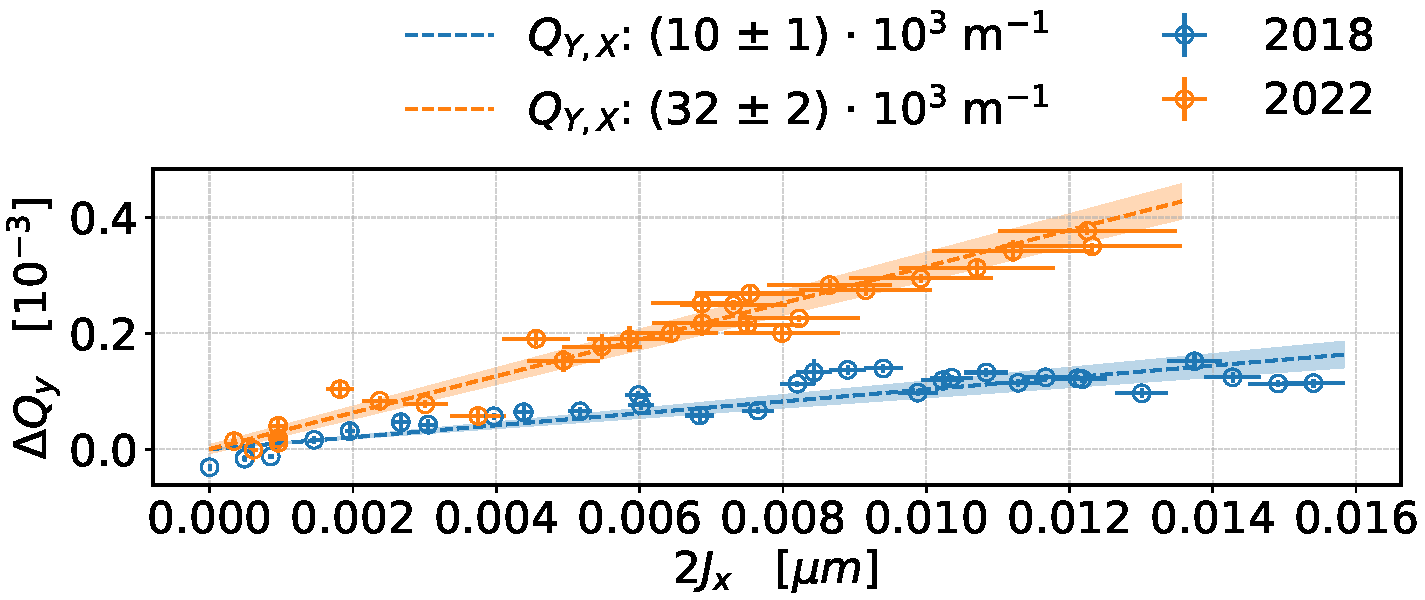
\includegraphics[width=0.5\linewidth]{images/nonlinear/comparison_2018_2022_dQYd2JX_corrected.pdf}
    \end{center}
    
    \begin{itemize}
        \item amplitude detuning larger than in run 2
        \item recomputing of IR non-linear correction necessary
    \end{itemize}
\end{frame}


% \backcover

\end{document}
